% ----------------------------------------------------
% -------- BAYSIS - Selected as Jam Follower ---------
% ----------------------------------------------------
\subsection{Congestion - Accidents categorizes as Jam Follower}
\label{analysis_processing_correlation_baysis_follower}
The correlation matrix table for the congestion - accident dataset, which are classified as \textit{Jam Follower} (see \cref{table:appendix_correlation_matrix_matched_cramers}) is visual presented in \cref{img:correlation_matrix_selected_effector_cramers} showing the the correlation of each variable combination. When visual analyzing \cref{img:correlation_matrix_matched_cramers} and checking the guidelines for a strong correlation in reference to the applied coefficient (identifiable with \cref{table:appendix_coefficient_matrix_matched}) we get a list of strongly correlated variable combinations (see \cref{tbl:correlation_list_baysis_follower}). Since the focus of the thesis are the correlations between accidents and jams, these are only collected from the bottom-left rectangle of the matrix, where the congestion and accidents variables intersect. Correlations of the kind congestion - congestion or accident - accident are not considered.
\begin{table}[h!]
	\centering
	\begin{tabular}{c|l}  
		Category & Strong \\
		\\[-1em]
		\hline
		\\[-1em]
		Strasse & TMax, TAvg, SMax, SAvg, TDist, SDist, Cov, TLHGV \\ 
 		Kat & TMax, SAvg \\ % + SMax % -> Strasse
 		%Typ & \\ + Cov % -> Strasse
 		%Betei & \\ % -> Strasse
 		UArt1 & TAvg, SAvg, TDist, Cov, TLHVG \\ % + SMax % -> Strasse
 		UArt2 & TDist \\ % + Cov % -> Strasse
 		AUrs1 & TDist, SDist, Cov, TLHGV \\ % -> Strasse
 		%AUrs2 & \\ % -> Strasse
 		AufHi & TMax, TAvg, Cov \\ % -> Strasse
 		%Alkoh & \\
 		%Char1 & \\ % -> Strasse
 		%Char2 & \\ % -> Strasse
 		Lich1 & Cov \\ % -> Strasse
 		%Lich2 & \\ + Cov % -> Strasse
 		%Zust1 & \\ + Cov % -> Strasse
 		%Zust2 & \\ % -> Strasse
 		%Fstf & \\ % -> Strasse
 		WoTag & TAvg, SMax, SAvg, TDist, Cov, TLHGV \\ % + TLCar % -> Strasse
 		%FeiTag & \\
 		Month & TMax, TAvg, SMax, Cov, TLHGV \\ % + SAvg % -> Strasse
	\end{tabular}
    \caption{List of incident variables and their strong correlated congestion variable from the congestion-accident matched data which are classified as \textit{Jam Follower}}
	\label{tbl:correlation_list_baysis_follower}
\end{table}
Next we need to verify that the correlation is significant and what the correlation predicates. Therefore each correlation will be evaluated with the Post Hoc test, defined in \cref{correlation_posthoc}. \secintroend{baysis}{follower}
\begin{figure}[!ht]
	\centering
	\makebox[\textwidth][c]{%
		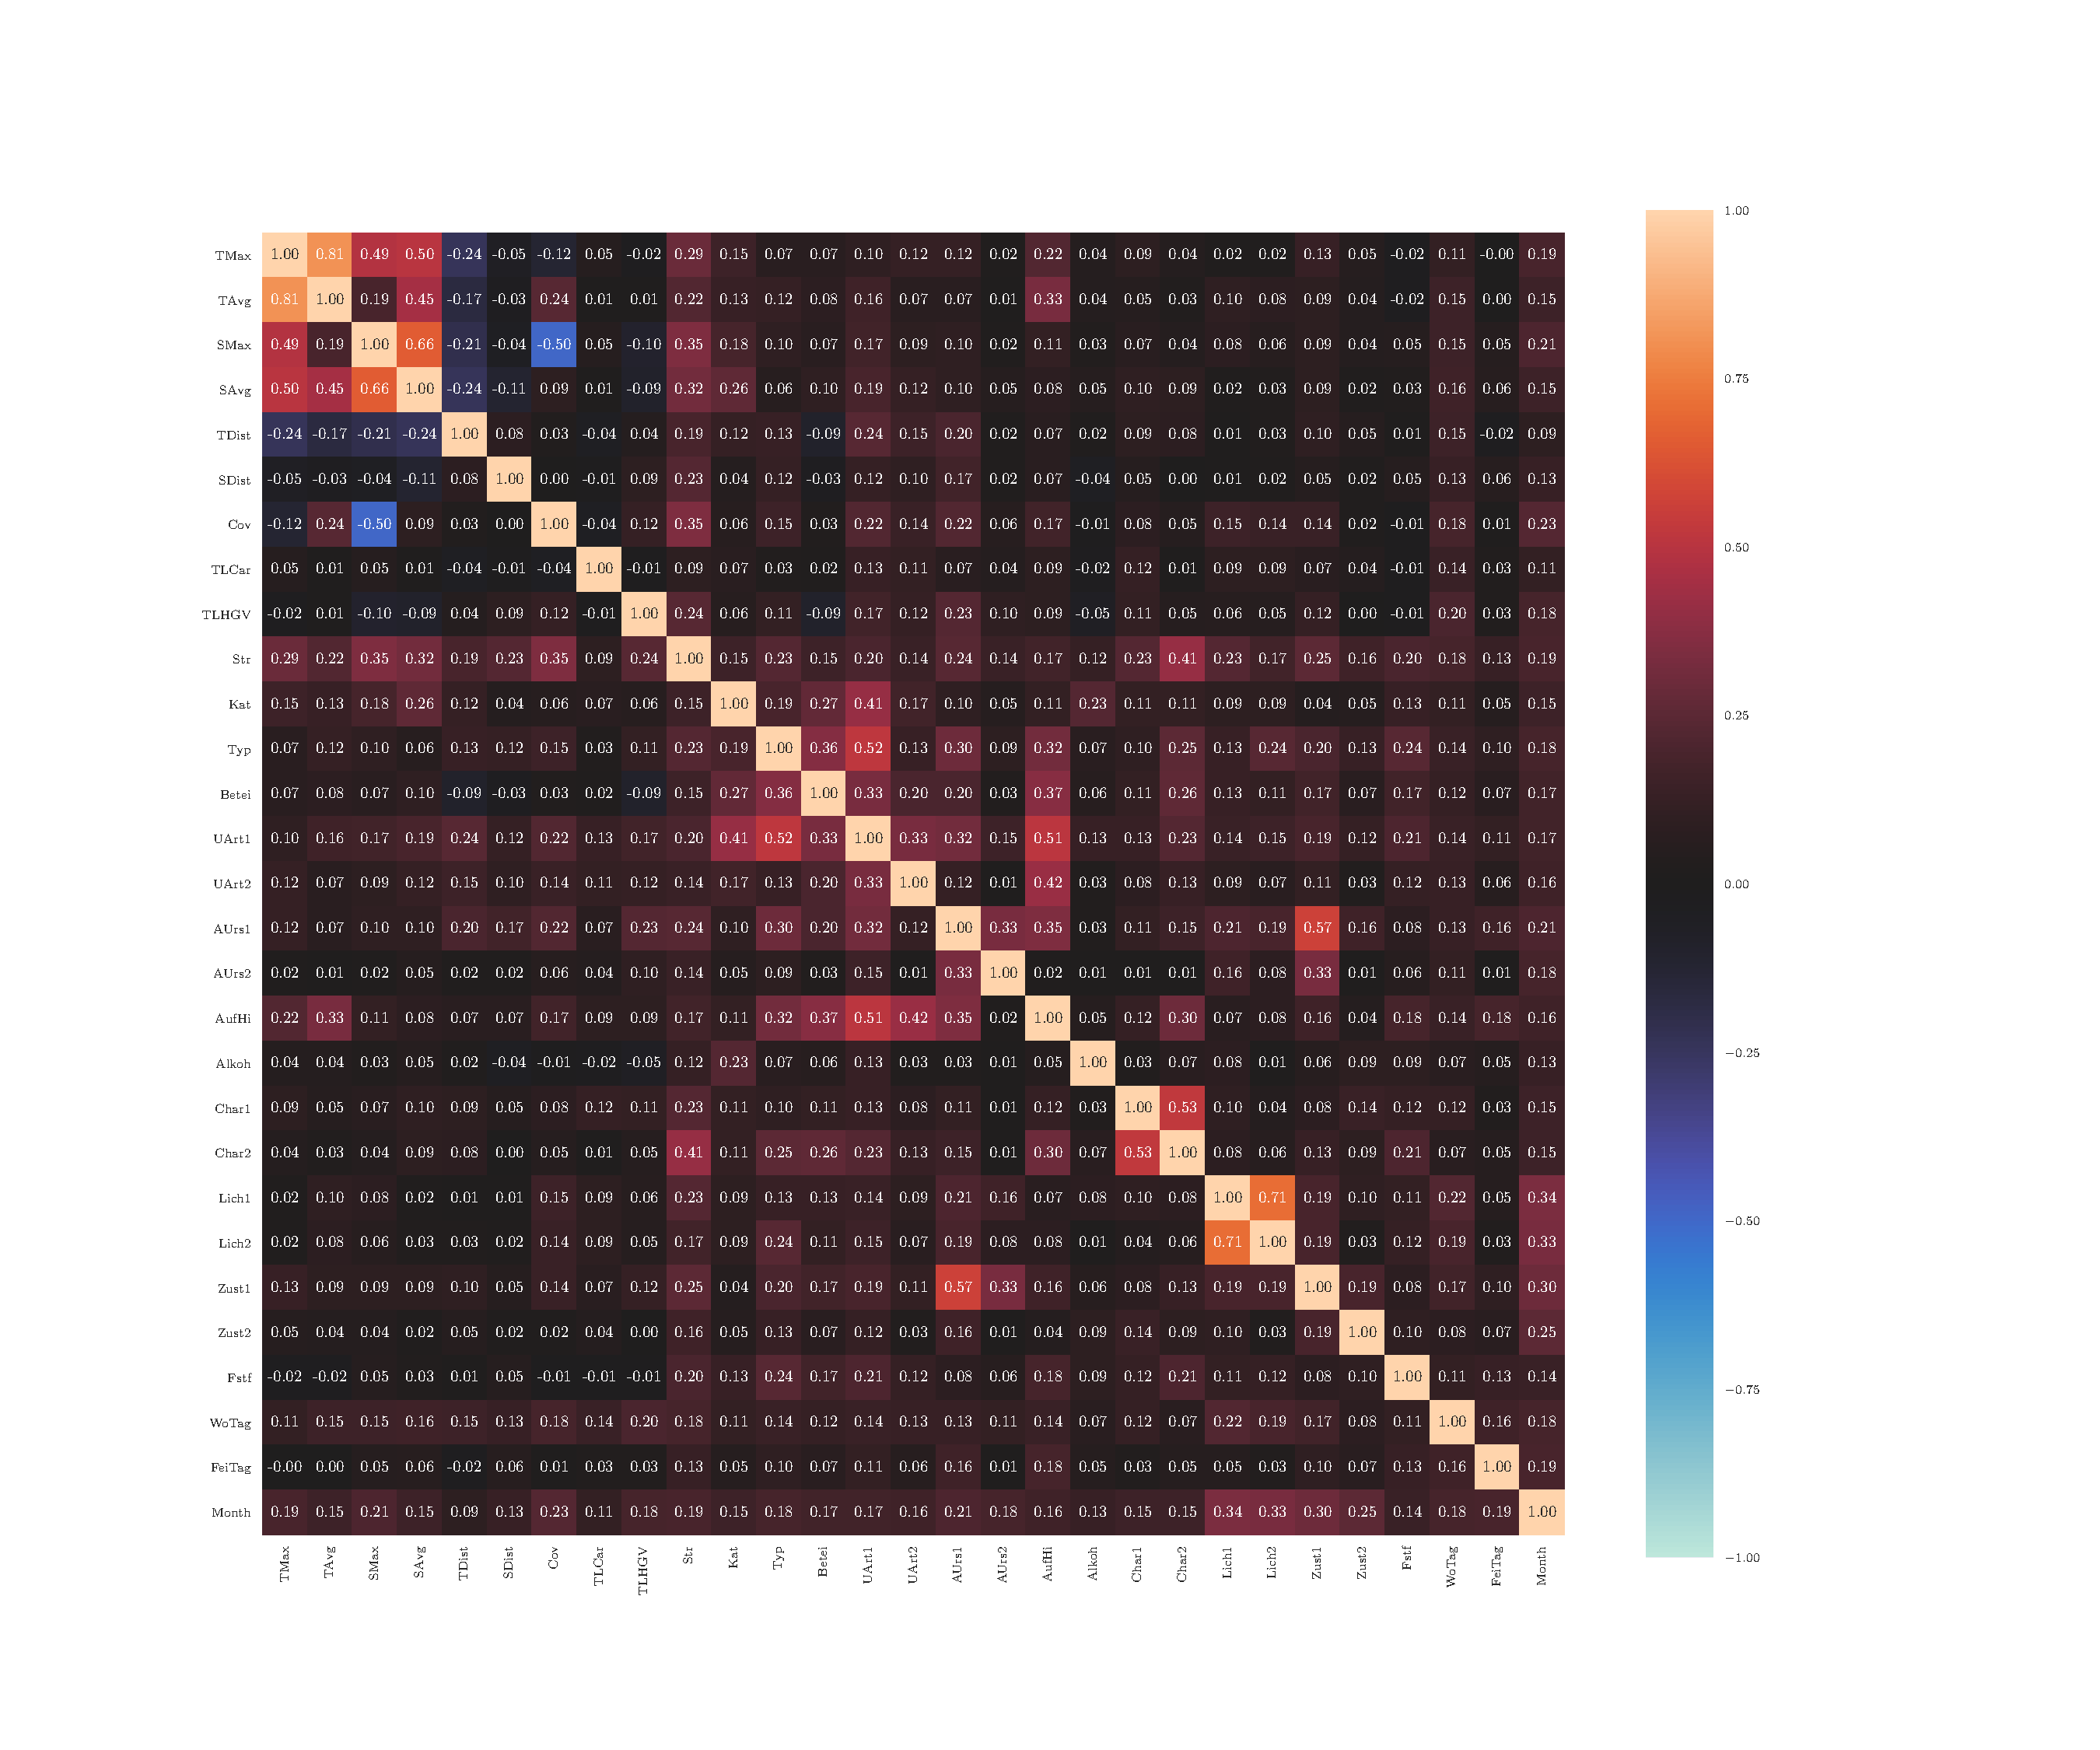
\includegraphics[width=1.4\textwidth, trim=0cm 2.5cm 6cm 3cm]{CorrAnalysis/data/BAYSIS/03_selected_03_endJam/plots/baysis_selected_corr_cramers}%
	}
	\caption{Correlation matrix for congestion-accident matched data classified as \textit{Jam Effector} and calculated with $V$, $\eta$, $\tau$, $r_{pq}$, $r$}
	\label{img:correlation_matrix_selected_effector_cramers}
\end{figure}

% --------------------------
% -------- Strasse ---------
% --------------------------
\centerheading{Strasse}
\varintronosigmul{Str}{\textit{Strasse} - \textit{TMax}, \textit{Strasse} - \textit{TAvg}, \textit{Strasse} - \textit{SMax}, \textit{Strasse} - \textit{SAvg}, \textit{Strasse} - \textit{TDist}, \textit{Strasse} - \textit{SDist}, \textit{Strasse} - \textit{Cov} and \textit{Strasse} - \textit{TLHGV}}

% ----------------------
% -------- Kat ---------
% ----------------------
\centerheading{Kat}
\varintronosigmul{Kat}{\textit{Kat} - \textit{TMax} and \textit{Kat} - \textit{SAvg}}

% ----------------------
% -------- Typ ---------
% ----------------------

% -----------------------
% -------- UArt ---------
% -----------------------
\centerheading{UArt}
\varintronosigmul{UArt}{\textit{UArt1} - \textit{TAvg}, \textit{UArt1} - \textit{SAvg}, \textit{UArt1} - \textit{TDist}, \textit{UArt1} - \textit{Cov}, \textit{UArt1} - \textit{TLHGV} and \textit{UArt2} - \textit{TDist}}

% -----------------------
% -------- AUrs ---------
% -----------------------
\centerheading{AUrs}
\varintrosimplewithsam{AUrs} \varintronosigmul{AUrs}{\textit{AUrs1} - \textit{TDist} and \textit{AUrs1} - \textit{TLHGV}}

% ##############################################
\groupintrosig{AUrs1}{SDist}{0.0372}{baysis}{follower}
It show shows that the significance differences is not group specific. The correlation can therefore be neglected.
% ######################## Expand if time ########################

% ##############################################
\groupintrosig{AUrs1}{Cov}{0.0372}{baysis}{follower}
It show shows that the significance differences is not group specific. The correlation can therefore be neglected.
% ######################## Expand if time ########################

% ------------------------
% -------- AufHi ---------
% ------------------------
\centerheading{AufHi}
\varintronosigmul{AufHi}{\textit{AufHi} - \textit{TMax}, \textit{AufHi} - \textit{TAvg} and \textit{AufHi} - \textit{Cov}}

% ------------------------
% -------- Lich1 ---------
% ------------------------
\centerheading{Lich}
\varintronosigsing{Lich1}{Cov}

% ------------------------
% -------- WoTag ---------
% ------------------------
\centerheading{WoTag}
\varintronosigmul{WoTag}{\textit{WoTag} - \textit{TMax}, \textit{WoTag} - \textit{SMax}, \textit{WoTag} - \textit{SAvg}, \textit{WoTag} - \textit{TDist}, \textit{WoTag} - \textit{Cov} and \textit{WoTag} - \textit{TLHGV}}

% ------------------------
% -------- Month ---------
% ------------------------
\centerheading{Month}
\varintronosigmul{Month}{\textit{Month} - \textit{TMax}, \textit{Month} - \textit{SMax}, \textit{Month} - \textit{SAvg}, \textit{Month} - \textit{Cov} and \textit{Month} - \textit{TLHGV}}
